% This is samplepaper.tex, a sample chapter demonstrating the
% LLNCS macro package for Springer Computer Science proceedings;
% Version 2.21 of 2022/01/12
%
\documentclass[runningheads]{llncs}
%
\usepackage[T1]{fontenc}
% T1 fonts will be used to generate the final print and online PDFs,
% so please use T1 fonts in your manuscript whenever possible.
% Other font encondings may result in incorrect characters.
%
\usepackage{graphicx}
\usepackage{multirow}
\usepackage[hidelinks]{hyperref}
% Used for displaying a sample figure. If possible, figure files should
% be included in EPS format.
%
% If you use the hyperref package, please uncomment the following two lines
% to display URLs in blue roman font according to Springer's eBook style:
%\usepackage{color}
%\renewcommand\UrlFont{\color{blue}\rmfamily}
%\urlstyle{rm}
%
\begin{document}
%
\title{Dance4Life: Plataforma de Sensorização para Envelhecimento Ativo através da Dança}
%
\titlerunning{Contribuição Sensorização e IA no Envelhecimento Ativo}
% If the paper title is too long for the running head, you can set
% an abbreviated paper title here
%
\author{
Carlos da Mota Bergueira (pg11605@alunos.uminho.pt) \\
Diego Jefferson Mendes Silva (pg59999@alunos.uminho.pt) \\
Filipa Araújo Pereira (pg42201@alunos.uminho.pt) \\
Rui Manuel Martins Marques Rodrigues (pg7942@alunos.uminho.pt)
}
%
\authorrunning{C. Bergueira, D. Silva, F. Pereira, R. Rodrigues}
% First names are abbreviated in the running head.
% If there are more than two authors, 'et al.' is used.
%
\institute{Universidade do Minho, Braga, Portugal \\
% \email{pg11605@alunos.uminho.pt, pg59999@alunos.uminho.pt, pg42201@alunos.uminho.pt, pg7942@alunos.uminho.pt}
}
%
\maketitle              % typeset the header of the contribution
%
\begin{abstract}
Este artigo apresenta o Dance4Life, uma plataforma de sensorização e inteligência artificial desenvolvida no âmbito da unidade curricular de Sensorização e Ambiente do Mestrado em Inteligência Artificial. O sistema tem como objetivo promover o envelhecimento ativo através da dança, integrando dados meteorológicos (OpenWeatherMap) com dados fisiológicos, inerciais e de localização recolhidos em dispositivos Android (smartphone e wearables). A arquitetura assenta em três pilares: um servidor Flask para ingestão e encaminhamento de dados, uma camada de agentes para processamento e persistência, e uma camada de visualização interativa com PowerBI e D3.js/Leaflet para análise exploratória. Em paralelo, os dados suportam o desenvolvimento de um agente de Aprendizagem por Reforço (RL), treinado em ambiente simulado estocástico (\texttt{MovementEnv}) com algoritmos DQN e PPO, para otimização de intervenções personalizadas. O trabalho demonstra a viabilidade de uma plataforma distribuída, centrada no utilizador sénior, que combina contexto ambiental, segurança fisiológica e motivação social através da música e da dança.

\keywords{Sensorização \and Dance4Life \and Envelhecimento Ativo \and Machine Learning \and HAR}
\end{abstract}
%
%
%
\section{Introdução}
O envelhecimento da população europeia constitui um dos maiores desafios sociais e de saúde pública do século XXI. Em Portugal, estima-se que, em 2050, mais de 35% da população terá mais de 65 anos, tornando imperativa a adoção de soluções tecnológicas que promovam a autonomia, a atividade física e a integração social da população sénior.
O Dance4Life surge como resposta a este desafio, propondo uma plataforma inteligente que combina sensorização ambiental e fisiológica com mecanismos de ludificação baseados na dança e na música. O sistema é concebido para funcionar em dispositivos móveis (smartphones e smartwatches), processando dados localmente segundo o paradigma de Edge Computing, em conformidade com os princípios de Privacy by Design exigidos pelo RGPD.
Este relatório documenta a segunda fase do trabalho prático, focada na implementação da plataforma: a definição e implementação dos coletores de dados, o tratamento e visualização dos dados recolhidos, e a conceção do agente de Aprendizagem por Reforço (RL) desenvolvido no contexto da unidade curricular de Aprendizagem por Reforço. Complementarmente, apresenta-se uma proposta de modelo de negócio que enquadra a viabilidade da solução em contextos reais.
O documento está organizado da seguinte forma: a Secção 2 descreve a arquitetura global do sistema e os domínios abordados; a Secção 3 detalha os sensores e os coletores de dados implementados; a Secção 4 apresenta a exploração e visualização dos dados; a Secção 5 descreve o agente de Aprendizagem por Reforço concebido; a Secção 6 analisa resultados e limitações; e a Secção 7 apresenta o modelo de negócio.

\section{Domínios, Objetivos e Arquitetura}
\subsection{Domínios Abordados}
O Dance4Life opera na intersecção de três domínios principais:
\subsubsection{Saúde e Bem-Estar Sénior} Monitorização da atividade física, frequência cardíaca e padrões de movimento, com o objetivo de promover o exercício seguro e personaliza-do.
\subsubsection{Ambiente Urbano Inteligente} Integração de dados contextuais do ambiente, com foco nas condições meteorológicas e de localização, para adaptar as recomendações de atividade ao contexto real do utilizador.
\subsubsection{Interação Social e Ludificação} Matching de utilizadores com perfis compatíveis (Dancing Match) e estímulos musicais adaptativos que transformam a monitorização passiva numa experiência ativa e motivadora.

\subsection{Objetivos}
Os objetivos da fase prática organizam-se em três níveis:
Implementar coletores de dados para sensores físicos e virtuais, integrando a API OpenWeatherMap e a recolha de dados em dispositivos Android (smartphone e wearables).
Explorar, tratar e visualizar os dados recolhidos, aplicando técnicas de visualização interativa com D3.js para análise de padrões temporais e correlações entre variáveis ambientais e fisiológicas.
Conceber e implementar um agente de Aprendizagem por Reforço (RL) para otimiza-ção da política de intervenção do sistema Dance4Life, equilibrando a promoção da atividade física com a prevenção de fadiga de alarme.

\subsection{Arquitetura Global do Sistema}
A arquitetura do Dance4Life segue um modelo distribuído em camadas, conforme ilustrado na Figura~\ref{arquitetura}. A camada de aquisição de dados agrega três tipos de fontes: dados meteorológicos (OpenWeatherMap), dados de sensores inerciais/fisiológicos dos dispositivos Android e dados de localização. Os dados convergem num servidor Flask central, responsável pela receção, validação, encaminhamento para agentes e persistência em base de dados. Uma camada de processamento alimenta o agente de Aprendizagem por Reforço responsável pelas decisões de intervenção. Por fim, uma camada de apresentação expõe dashboards interativos com PowerBI,D3.js e Leaflet para análise exploratória dos dados.

\begin{figure}
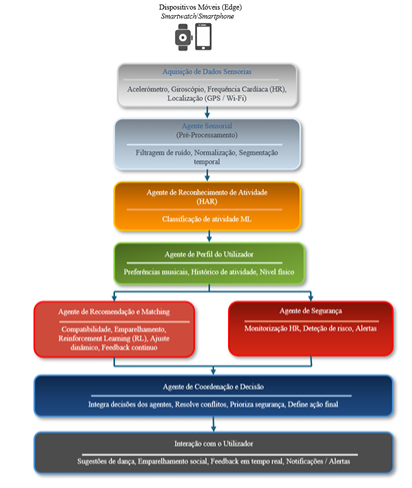
\includegraphics[width=\textwidth]{images/arquitetura.png}
\caption{Arquitetura global do sistema Dance4Life.} \label{arquitetura}
\end{figure}

A separação entre a camada de Edge (dispositivos móveis) e a camada de servidor garante que os dados biométricos granulares são processados localmente, transmitindo apenas inferências categóricas anonimizadas para o servidor central, em conformidade com o RGPD.

\section{Sensores, Coletores de Dados e Ambiente}

\subsection{Sensores Virtuais Ambientais}
Na implementação atual, o contexto ambiental é obtido através de um módulo de sensorização virtual meteorológica. Este sensor permite ao sistema adaptar recomendações de atividade em função das condições climáticas no momento da recolha.

\subsubsection{Sensor Meteorológico (OpenWeatherMap)}
O módulo external\_sensors.py recolhe dados meteorológicos em tempo real, recorrendo à API REST da OpenWeatherMap (endpoint \texttt{/data/2.5/weather}). A consulta pode ser realizada por coordenadas geográficas (latitude/longitude) ou por cidade. Os parâmetros recolhidos incluem temperatura (\(^\circ\)C), humidade relativa (\%), velocidade do vento (m/s) e timestamp Unix da observação. Os dados são obtidos em unidades métricas (\texttt{units=metric}) e retornados como dicionário Python, facilitando a integração com os restantes módulos.
A relevância deste sensor para o Dance4Life reside na capacidade de contextualizar a atividade física: temperaturas extremas ou humidade elevada condicionam a intensida-de recomendada pelo sistema, enquanto condições favoráveis podem ser utilizadas como estímulo adicional para atividade ao ar livre.
\subsubsection{Simulador Dispositivo Android}
O módulo \_simulate\_android\_emulator.py replica o comportamento de um dispositivo Android equipado com sensores inerciais e fisiológicos, enviando dados simulados para o servidor Flask através de pedidos HTTP POST. Cada payload gerado inclui um identificador de utilizador (\texttt{user\_1} a \texttt{user\_5}), leituras de acelerómetro (\texttt{acc}, normalizado entre 0 e 1), frequência cardíaca (\texttt{hr}, entre 60 e 160 bpm), ritmo de movimento (\texttt{ritmo}, entre 0 e 1), coordenadas GPS (\texttt{latitude} e \texttt{longitude}, na região do Porto) e timestamp UTC.
A geração de dados segue uma distribuição aleatória uniforme, o que permite testar o comportamento do sistema em condições diversas de atividade. Os dados são envia-dos com um intervalo de 30 segundos, simulando a cadência de amostragem de um dispositivo real em contexto de monitorização contínua. O mecanismo de timeout configurado (3 segundos de ligação, 20 segundos de leitura) garante robustez perante latências do servidor.
O endpoint de receção (\texttt{/collect\_data\_activities}) foi configurado no servidor Flask local (localhost:5000), com suporte para endereçamento alternativo em rede local, facilitando testes em cenários de dispositivos fisicamente distribuídos.


\subsection{Servidor de Recolha de Dados (Flask)}
O servidor Flask constitui o núcleo da camada de recolha de dados, expondo endpoints REST para receção dos dados provenientes do simulador Android e para consulta dos dados ambientais recolhidos pelos sensores virtuais. A arquitetura do servidor segue o padrão MVC simplificado, com separação entre a lógica de receção de dados, a camada de persistência em base de dados e os módulos de sensorização.
A cada pedido recebido no endpoint \texttt{/collect\_data\_activities}, o servidor valida o payload JSON, adiciona metadados temporais e encaminha os dados para os agentes de processamento (HAR, ambiente, base de dados, coordenador e matching). O enriquecimento ambiental, aplicado em tempo de execução, centra-se na variável de temperatura. Esta fusão de dados sensoriais e contextuais numa operação de ingestão integrada constitui um dos elementos distintivos da arquitetura Dance4Life.

\begin{figure}
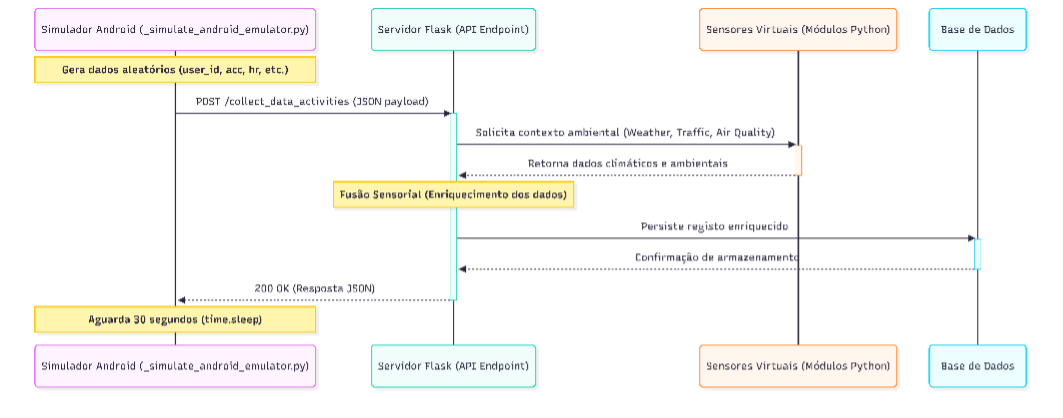
\includegraphics[width=\textwidth]{images/diagrama-fluxo.png}
\caption{Diagrama de sequência do fluxo de recolha de dados.} \label{diagrama_fluxo}
\end{figure}

\section{Exploração e Visualização dos Dados}
\subsection{Tratamento e Pré-Processamento}

Na implementação atual, o tratamento de dados ocorre em duas fases complementares:
\subsubsection{Validação e enriquecimento em ingestão} no servidor Flask, cada payload recebido é validado a nível estrutural (JSON válido e campos esperados), enriquecido com metadados temporais e encaminhado para os agentes de processamento.
\subsubsection{Agregação para análise} no dashboard PowerBI/D3.js, os dados persistidos são agregados por utilizador, mês, cidade e estado de convite, permitindo análise exploratória comparativa e cálculo de indicadores de participação (atividade, convites aceites, matching e recomendações).

\subsection{Análise Exploratória}
A análise exploratória dos dados recolhidos focou-se na identificação de padrões temporais e comportamentais de utilização da plataforma. A distribuição de atividade por utilizador permitiu distinguir perfis de maior e menor participação, enquanto a análise temporal mensal evidenciou variações no volume de recolha ao longo do período observado. A análise por cidade, suportada por visualização georreferenciada, permitiu identificar concentração de atividade em determinados contextos geográficos. Adicionalmente, a distribuição de estados de convite (aceite, recusado, pendente) e os indicadores de matching forneceram uma perspetiva complementar sobre o envolvimento social promovido pelo sistema.

\begin{figure}
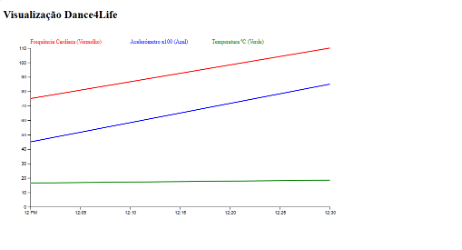
\includegraphics[width=\textwidth]{images/serie-temporal.png}
\caption{Séries temporais das variáveis sensoriais recolhidas (D3.js).} \label{serie_temporal}
\end{figure}

\subsection{Técnicas de Visualização Implementadas}
As visualizações foram implementadas recorrendo à biblioteca D3.js, escolhida pela sua flexibilidade e capacidade de renderização interativa de grandes volumes de dados temporais. Foram desenvolvidos os seguintes tipos de visualização:

\begin{itemize}
\item Gráfico de barras (Top 10): comparação dos utilizadores com melhor score global, agregando atividade, convites aceites, matching e recomendações.
\item Série temporal mensal (line chart): evolução do número de registos de atividade ao longo do tempo.
\item Mapa por cidade (Leaflet + D3): distribuição geográfica da atividade, com codificação visual por intensidade de registos.
\item Distribuição de convites por estado: visualização comparativa entre convites aceites, recusados e pendentes.
\item Cartão individual de utilizador com gráfico circular: decomposição do score por componentes de participação.
\end{itemize}

\begin{figure}
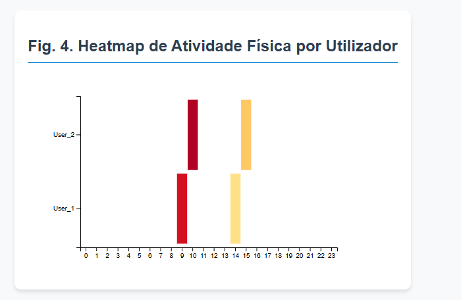
\includegraphics[width=\textwidth]{images/heatmap-atividades.png}
\caption{Visualização de intensidade de atividade no dashboard (D3.js).} \label{heatmap_atividade}
\end{figure}

\section{Modelos de Machine Learning}
O motor de decisão inteligente do Dance4Life é implementado através de um agente de Aprendizagem por Reforço (RL), desenvolvido no âmbito da unidade curricular de Aprendizagem por Reforço do Mestrado em Inteligência Artificial. O agente é responsável por aprender uma política ótima de intervenção, decidindo em cada momento quando e com que intensidade intervir junto do utilizador sénior, equilibrando dois objetivos críticos em geriatria: a promoção da atividade física (combate ao sedentarismo) e a preservação do bem-estar psicológico (prevenção de fadiga de alarme e rejeição tecnológica).

\subsection{Problema de Classificação e Classes}
O problema é formalmente modelado como um Processo de Decisão de Markov (MDP), estruturado da seguinte forma:
\subsubsection{Espaço de Estado} O espaço de observação é contínuo, composto por três variáveis dinâmicas com valores no intervalo [0, 10], que representam o estado multidimensional do utilizador em cada instante temporal:

\begin{table}
\centering
\caption{Espaço de estado do MDP do agente Dance4Life.}\label{estados_mdp}
\begin{tabular}{|l|c|p{6.6cm}|}
\hline
Variável de Estado &  Intervalo & Descrição\\
\hline
Nível de Atividade &  [0, 10] & Grau atual de movimento do utilizador (0 = sedentarismo absoluto)\\
Fadiga Física &  [0, 10] & Cansaço fisiológico/cardíaco acumulado ao longo da sessão\\
Irritação (Fadiga de Alarme) &  [0, 10] & Saturação psicológica pelas notificações enviadas pelo sistema\\
\hline
\end{tabular}
\end{table}

\subsubsection{Espaço de Ação}
O espaço de ação é discreto, com quatro níveis de intensidade de intervenção que o agente pode selecionar em cada timestep:

\begin{itemize}
\item Ação 0 — Silêncio: Nenhuma intervenção. Prioriza o descanso e reduz a irri-tação, mas conduz à queda progressiva do nível de atividade.
\item Ação 1 — Baixa Intensidade: Incentivo leve (ex.: notificação suave ou suges-tão musical subtil). Mantém o nível de atividade base e apoia a recuperação, com ligeiro incremento da irritação.
\item Ação 2 — Média Intensidade: Recomendação moderada (ex.: sugestão de sessão de dança leve). Aumenta a atividade para níveis saudáveis, com in-cremento equilibrado de fadiga e irritação.
\item Ação 3 — Alta Intensidade: Desafio forte (ex.: convite a sessão de dança ati-va com parceiro). Maximiza a atividade em casos críticos de sedentarismo, mas com custo elevado em fadiga e irritação.
\end{itemize}

\subsubsection{Função de Recompensa}
A função de recompensa foi cuidadosamente desenhada para codificar os objetivos clínicos e comportamentais do sistema, penalizando estados de risco e recompensando a manutenção do utilizador na zona de atividade ideal:

\begin{table}
\centering
\caption{Função de recompensa do agente de Aprendizagem por Reforço.}\label{recompensa_mdp}
\begin{tabular}{|l|p{9.7cm}|}
\hline
Recompensa &  Condição e Descrição\\
\hline
+15 (contí-nua) &  Utilizador na zona ideal: Atividade ∈ [4, 7], Fadiga < 7 e Irritação < 5\\
-5 (contí-nua) &  Utilizador em sedentarismo perigoso: Atividade < 2 por timestep\\
-50 (termi-nal) &  Estado de Game Over: Fadiga Máxima (risco médico) OU Irrita-ção Máxima (abandono do sistema)\\
\hline
\end{tabular}
\end{table}

A penalização terminal de -50 é particularmente relevante: modela dois cenários de falha crítica distintos — o risco médico por exaustão fisiológica e o abandono tecno-lógico por fadiga de alarme — ambos determinando o fim do episódio. Esta dualida-de obriga o agente a aprender uma política equilibrada que não apenas maximize a atividade, mas também gerencie ativamente a saturação psicológica do utilizador.

\subsection{Ambiente Simulado — MovementEnv}
Devido às restrições éticas que impedem o treino inicial com utilizadores reais (população sénior vulnerável), o agente é treinado num ambiente simulado estocástico designado \texttt{MovementEnv}, desenvolvido com a framework Gymnasium da Farama Foundation. Este ambiente imita a evolução fisiológica e comportamental de um utilizador idoso, gerando estados dinâmicos e reagindo às intervenções do agente de forma realista.
O ambiente incorpora estocasticidade nas transições de estado, modelando a variabilidade natural do comportamento humano: a mesma ação do agente pode produzir respostas ligeiramente diferentes em diferentes episódios, replicando a imprevisibilidade inerente a utilizadores reais. A integração com o ecossistema Dance4Life permite que os dados ambientais recolhidos pelos sensores virtuais (temperatura, qualidade do ar) influenciem os parâmetros de transição do ambiente simulado, enriquecendo o realismo da simulação.

\begin{figure}
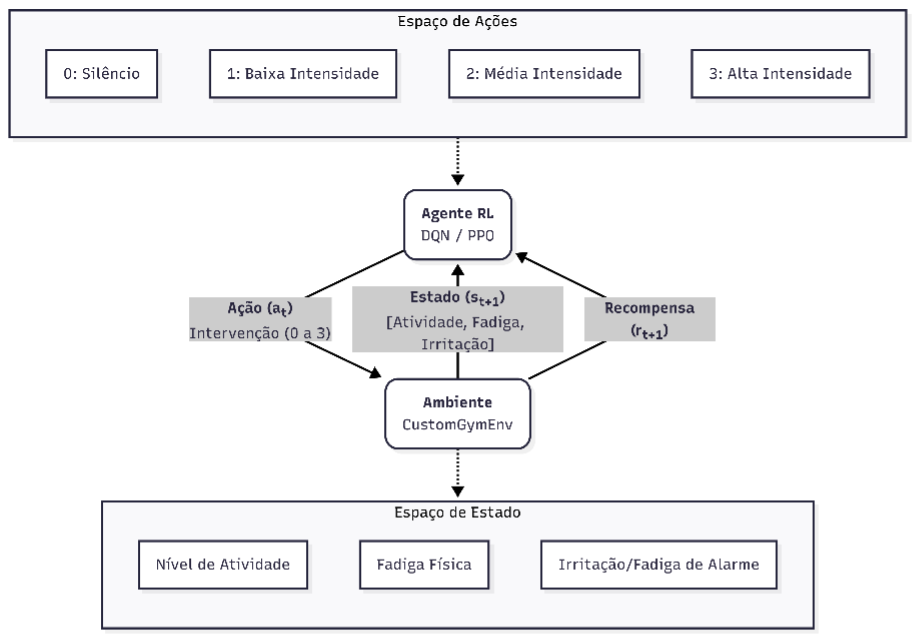
\includegraphics[width=\textwidth]{images/ciclo-rl.png}
\caption{Ciclo de interação do agente RL com o ambiente \texttt{MovementEnv}.} \label{ciclo_rl}
\end{figure}

\subsection{Algoritmos Implementados: DQN e PPO}
Foram implementados e avaliados comparativamente dois algoritmos de Deep Reinforcement Learning, selecionados pela sua adequação às características do problema (estados contínuos, ações discretas), recorrendo à biblioteca Stable-Baselines3.
\subsubsection{DQN — Deep Q-Network} O DQN é um algoritmo baseado em valor (value-based) que aproxima a função Q(s, a) — o valor esperado de executar a ação a no estado s — através de uma rede neuronal profunda. Utiliza dois mecanismos fundamentais para estabilizar o treino em ambientes com estados contínuos: Experience Replay (armazenamento e amostragem aleatória de experiências passadas para quebrar correlações temporais) e Target Network (rede alvo de atualização lenta para evitar oscilações na função de valor). A sua natureza value-based torna-o particularmente adequado para espaços de ação discretos como o definido no MDP Dance4Life.
\subsubsection{PPO — Proximal Policy Optimization} O PPO é um algoritmo baseado em política (policy-based/actor-critic), reconhecido no estado da arte pela sua estabilidade de treino e facilidade de convergência. O mecanismo central do PPO é a função objetivo clipped surrogate, que limita a magnitude das atualizações de política a cada iteração, evitando passos de gradiente demasiado grandes que poderiam desestabilizar o agente. A componente critic estima o valor do estado atual, guiando as atualizações da componente actor (a política propriamente dita). A robustez do PPO em ambientes estocásticos torna-o o candidato preferencial para o cenário Dance4Life.

\subsection{Métricas de Avaliação e Comparação}
A avaliação e comparação dos dois agentes (DQN vs. PPO) é realizada através das seguintes métricas:
\subsubsection{Curvas de Aprendizagem} evolução da recompensa média por episódio ao longo dos timesteps de treino, permitindo avaliar a velocidade de convergência e a estabilidade de cada algoritmo.
\subsubsection{Duração Média dos Episódios} capacidade do agente para manter o utilizador ativo ao longo de uma sessão completa sem desencadear um estado terminal (Game Over por fadiga ou abandono).
\subsubsection{Survival Rate} proporção de episódios concluídos com sucesso total, sem atingir nenhum dos limites críticos definidos na função de recompensa.
\subsubsection{Análise Comparativa de Política}  exame das políticas aprendidas por cada agente — quais ações são preferidas em que estados — para avaliar a adequação clínica das deci-sões tomadas.

\begin{table}
\centering
\caption{Comparação de desempenho DQN vs. PPO no ambiente \texttt{MovementEnv}.}\label{comparacao_algoritmos}
\begin{tabular}{|l|l|l|}
\hline
Métrica & DQN & PPO\\
\hline
Recompensa Média (30 episódios) &  1437.50 & 1436.00\\
Duração Média de Episódio (passos) &  96.00 & 96.00\\
Survival Rate &  100.00\% & 100.00\%\\
Timesteps até melhor desempenho observado &  20\,000 & 260\,000\\
\hline
\end{tabular}
\end{table}

\section{Resultados, Limitações e Recomendações}
\subsection{Sumário dos Resultados Obtidos}
A implementação da plataforma Dance4Life na sua fase prática permitiu alcançar os seguintes resultados:

\begin{itemize}
\item Integração do sensor virtual meteorológico (OpenWeatherMap), com recolha contínua de dados ambientais para suporte contextual.
\item Implementação de um simulador de dispositivo Android funcional, capaz de gerar e transmitir dados fisiológicos e inerciais realistas para o servidor Flask com intervalo de 30 segundos.
\item Desenvolvimento de um servidor Flask robusto, com mecanismo de fusão sensorial na ingestão e persistência em base de dados rela-cional.
\item Criação de um conjunto de visualizações PowerBI e D3.js/Leaflet interativas que permitem a análise exploratória dos dados recolhidos, incluindo ranking, série temporal, distribuição geográfica e estado de convites.
\item Conceção e avaliação comparativa de dois agentes de Aprendizagem por Reforço (DQN e PPO) num ambiente simulado estocástico (\texttt{MovementEnv}), com formulação MDP documentada e métricas de avaliação definidas.
\end{itemize}

\subsection{Análise Crítica e Limitações}
A principal limitação da implementação atual reside na utilização exclusiva de dados simulados — tanto para os sensores inerciais e fisiológicos como para o ambiente de treino do agente RL (\texttt{MovementEnv}). Os dados gerados seguem distribuições estocásticas parametrizadas que, embora mais realistas do que distribuições uniformes simples, não capturam a plena complexidade e variabilidade real dos padrões fisiológicos e comportamentais de utilizadores seniores. Esta limitação condiciona a capacidade de generalização da política aprendida pelo agente para contextos do mundo real.
Uma limitação adicional reside na cobertura ambiental ainda centrada em variáveis meteorológicas, o que reduz a representatividade de contexto face a cenários urbanos mais complexos. Do ponto de vista do agente RL, a estocasticidade do ambiente \texttt{MovementEnv} introduz variância nas estimativas de recompensa durante o treino. Na avaliação comparativa realizada (30 episódios), ambos os modelos apresentaram survival rate de 100\% e duração média de 96 passos por episódio; o DQN obteve recompensa média ligeiramente superior, enquanto o PPO mostrou comportamento igualmente estável. Estes resultados sugerem desempenho robusto dos dois métodos no ambiente simulado, carecendo ainda de validação com dados reais.

\subsection{Recomendações para Trabalho Futuro}
Com base na análise crítica realizada, identificam-se as seguintes recomendações para o desenvolvimento futuro da plataforma:
\begin{itemize}
\item Validação do agente RL com utilizadores reais ou com dados recolhidos de voluntários, substituindo gradualmente o \texttt{MovementEnv} por um ambiente de simulação calibrado com dados empíricos reais de população sénior.
\item Extensão do espaço de estado do MDP com variáveis contextuais adicionais, permitindo ao agente adaptar as intervenções ao contexto ambiental em tempo real de forma mais robusta.
\item Implementação do paradigma de Federated Learning para personalização distribuída da política do agente, preservando a privacidade e adaptando as intervenções às características biomecânicas individuais de cada utilizador.
\item Integração de um módulo de inferência implícita de preferências musicais, correlacionando os dados de acelerómetro com as músicas reproduzidas, para enriquecer o espaço de ação do agente com recomendações musicais personalizadas.
\item Desenvolvimento de uma interface móvel nativa (Android/iOS) para substituição gradual do simulador e testes em condições reais de utilização.
\end{itemize}

\section{Modelo de Negócio}
\subsection{Proposta de Valor e Cliente-Alvo}
O Dance4Life posiciona-se como uma plataforma B2B2C (Business-to-Business-to-Consumer), cujo cliente primário são instituições de cuidado sénior — centros de dia, lares de idosos e programas municipais de envelhecimento ativo — e cujo utilizador final é a população sénior (65+ anos). A proposta de valor diferencia-se em três eixos: personalização baseada em dados (adaptação da atividade e da música ao perfil individual), segurança fisiológica (monitorização da frequência cardíaca e alertas em tempo real), e combate ao isolamento social (emparelhamento social — Dancing Match).

\subsection{Parcerias Estratégicas}
A viabilidade do Dance4Life assenta num ecossistema de parcerias estratégicas:
\begin{itemize}
\item Instituições de saúde e cuidado sénior: parceiros de distribuição e validação clínica (ex.: Santa Casa da Misericórdia, SCML, Misericórdias locais).
\item Fabricantes de wearables: integração nativa com dispositivos como Fitbit, Garmin ou Apple Watch para acesso a dados fisiológicos reais de alta qualidade.
\item Serviços de streaming musical: licenciamento de conteúdo musical adaptado (ex.: Spotify API, TIDAL) para alimentar o motor de recomendação musical.
\item Municípios e programas de saúde pública: parceiros de financiamento no contexto de cidades inteligentes e políticas de envelhecimento ativo.
\end{itemize}

\subsection{Estratégia de Monetização}
A estratégia de monetização combina dois modelos complementares:
\begin{itemize}
\item Subscrição institucional (SaaS): licença mensal por instituição, com preço escalável em função do número de utilizadores ativos. Este modelo garante receita recorrente e previsível.
\item Modelo freemium para utilizadores individuais: versão gratuita com funcionalidades básicas (monitorização de atividade e sugestões musicais), e versão premium com funcionalidades avançadas (em-parelhamento social, relatórios de saúde detalhados, integração com wearables).
\end{itemize}

Adicionalmente, os dados anonimizados e agregados gerados pela plataforma constituem um ativo de valor para investigação académica e para entidades de saúde pública, abrindo uma terceira linha de receita através de parcerias de investigação e venda de insights analíticos, sempre em conformidade com o RGPD.

\section{Conclusão}
O presente trabalho documentou o desenvolvimento da fase prática do projeto Dance4Life, uma plataforma de sensorização e inteligência artificial para a promoção do envelhecimento ativo através da dança. A implementação demonstrou a viabilidade técnica da integração de dados meteorológicos (OpenWeatherMap) com dados de dispositivos Android (smartphone e wearables), num servidor Flask capaz de realizar ingestão, encaminhamento por agentes e persistência em tempo real.
A exploração dos dados recolhidos através de visualizações PowerBI e D3.js/Leaflet revelou padrões temporais, geográficos e de participação social úteis para monitorização do sistema. O agente de Aprendizagem por Reforço concebido — com formulação MDP e implementação comparativa de DQN e PPO — constitui o motor de decisão inteligente da plataforma, capaz de aprender políticas de intervenção que equilibram atividade física e bem-estar psicológico.
O Dance4Life demonstra como a convergência de sensorização ambiental, processamento inteligente e ludificação pode criar uma solução tecnológica diferenciada para um dos maiores desafios sociais contemporâneos: o envelhecimento ativo. A proposta de modelo de negócio delineada reforça a viabilidade da solução em contextos reais, abrindo caminho para uma implementação piloto em parceria com instituições de cuidado sénior.
Como trabalho futuro, a prioridade recai na substituição dos dados simulados por dados reais de utilizadores seniores e na implementação do módulo de Aprendizagem Federada, que permitirá ao sistema aprender de forma distribuída e privacidade-preservante, completando a visão de um sistema verdadeiramente inteligente, adaptativo e centrado no utilizador.

% ---- Bibliography ----
%
% BibTeX users should specify bibliography style 'splncs04'.
% References will then be sorted and formatted in the correct style.
%
% \bibliographystyle{splncs04}
% \bibliography{mybibliography}
%
\begin{thebibliography}{11}

\bibitem{bouchabou2021}
Bouchabou, D., Nguyen, S.M., Lohr, C., LeDuc, B., Kanellos, I.: A Survey of Human Activity Recognition in Smart Homes Based on IoT Sensors Algorithms. Sensors \textbf{21}(18), 6037 (2021).

\bibitem{liu2024}
Liu, C., Thiamwong, L., Nguyen, T., Suarez, J.R., Park, J.-H., Lou, Q., Xie, R.: A reinforcement learning approach to enhance physical activity and reduce fall risk in older adults. Innovation in Aging 8(Suppl.~1), 1081--1081 (2024). \doi{10.1093/geroni/igae098.3473}

\bibitem{gonul2021}
Gönül, S., Namlı, T., Coşar, A., Toroslu, I.H.: A reinforcement learning based algorithm for personalization of digital, just-in-time, adaptive interventions. Artificial Intelligence in Medicine 115, 102062 (2021). \doi{10.1016/j.artmed.2021.102062}

\bibitem{hossen2025}
Hossen, M.A., Abas, P.E.: Machine Learning for Human Activity Recognition: State-of-the-Art Techniques and Emerging Trends. J. Imaging 11(3), 91 (2025).

\bibitem{liao2019}
Liao, P. et al.: Personalized HeartSteps: A Reinforcement Learning Algorithm for Optimizing Physical Activity. ACM (2019). \doi{10.1145/3381007}

\bibitem{lu2024}
Lu, Y. et al.: StepCountJITAI: simulation environment for RL with application to physical activity adaptive intervention. arXiv:2411.00336 (2024).

\bibitem{paraschiakos2020}
Paraschiakos, S. et al.: Activity recognition using wearable sensors for tracking the elderly. User Model. User-Adapt. Interact. \textbf{30}, 567--605 (2020).

\bibitem{peng2024}
Peng, C. et al.: Promoting physical activity in middle-aged and older adults through digital intervention via deep reinforcement learning. Int. J. Human-Computer Interaction (2024). \doi{10.1080/23311908.2025.2541720}

\bibitem{gymnasium_url}
Gymnasium (Farama Foundation): Framework para ambientes de Aprendizagem por Reforço. \url{https://gymnasium.farama.org/} (acedido em maio de 2026).

\bibitem{sb3_url}
Stable-Baselines3: Biblioteca de algoritmos de Deep RL em PyTorch. \url{https://stable-baselines3.readthedocs.io/} (acedido em maio de 2026).

\bibitem{openweathermap_url}
OpenWeatherMap API Documentation. \url{https://openweathermap.org/api} (acedido em maio de 2026).

\end{thebibliography}
\end{document}
